\documentclass{article}
\usepackage{tikz, comment}
\usepackage{pifont}
\usepackage{fontspec, pgfplots}
\usetikzlibrary{arrows, decorations.markings, decorations.pathreplacing}
\begin{comment}
:Title: Not defined yet
:Tags: joint variation, jointly proportional;focus of a parabola;focal radius ;synthetic substitution;moment
:Prob: 0.4491;0.4389;0.4316;0.4279;0.4278
:Author: Prof.Hu Ji-shan, HKUST
:Slug: No name yet

Description Here.........
\end{comment}
\begin{document}\centering 

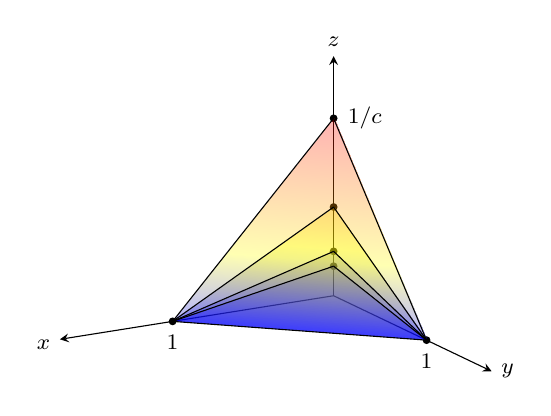
\begin{tikzpicture}[font=\footnotesize]
\pgfplotsset{compat=1.8}
\begin{axis}
[axis lines = center, view={150}{20}, ticks=none, scale=0.8,
axis background, xlabel = {$x$}, ylabel ={$y$}, zlabel ={$z$}, domain =-2:2, y domain =-2:2,
xmin =0,
xmax =1.7,
ymin =0,
ymax =1.7,
zmin =0, 
zmax =2.7,
samples =10, samples y =40, z buffer = auto, 
every axis x label/.style={
    at={(ticklabel* cs:1)},
    anchor= east, yshift =-2
},
every axis y label/.style={
    at={(ticklabel* cs:1)},
    anchor= west,
},
every axis z label/.style={
    at={(ticklabel* cs:1)},
    anchor= south
}]

\node[label={-90:{$1$}},circle,fill,inner sep=1pt] at (axis cs:1,0,0) {};		
\node[label={-90:{$1$}},circle,fill,inner sep=1pt] at (axis cs:0,1,0) {};		
\node[label={0:{$1/c$}},circle,fill,inner sep=1pt] at (axis cs:0,0,2) {};	
\node[label={5:{}},circle,fill,inner sep=1pt] at (axis cs:0,0,1) {};	
\node[label={5:{}},circle,fill,inner sep=1pt] at (axis cs:0,0,0.5) {};	
\node[label={5:{}},circle,fill,inner sep=1pt] at (axis cs:0,0,0.333) {};	

\addplot3[surf, shader=interp, mesh/cols=2, opacity=0.3] coordinates
		{(1,0,0) (0,1,0) (0,0,{1/(1/2)}) (0,0,{1/(1/2)})};

\addplot3[surf, shader=interp, mesh/cols=2, opacity=0.3] coordinates
		{(1,0,0) (0,1,0) (0,0,1) (0,0,1)};

\addplot3[surf, shader=interp, mesh/cols=2, opacity=0.3] coordinates
		{(1,0,0) (0,1,0) (0,0,1/2) (0,0,1/2)};

\addplot3[surf, shader=interp, mesh/cols=2, opacity=0.3] coordinates
		{(1,0,0) (0,1,0) (0,0,1/3) (0,0,1/3)};

\addplot3[surf, black] coordinates
		{(1,0,0) (0,1,0) (0,0,2) (1,0,0)};

\addplot3[surf, black] coordinates
		{(0,1,0) (0,0,1) (1,0,0)};

\addplot3[surf, black] coordinates
		{(0,1,0) (0,0,1/2) (1,0,0)};

\addplot3[surf, black] coordinates
		{(0,1,0) (0,0,1/3) (1,0,0)};
		
\end{axis}

\end{tikzpicture}
\end{document}